
\chapter{\pricewars Platform}

\begin{figure}[h]
	\centering
	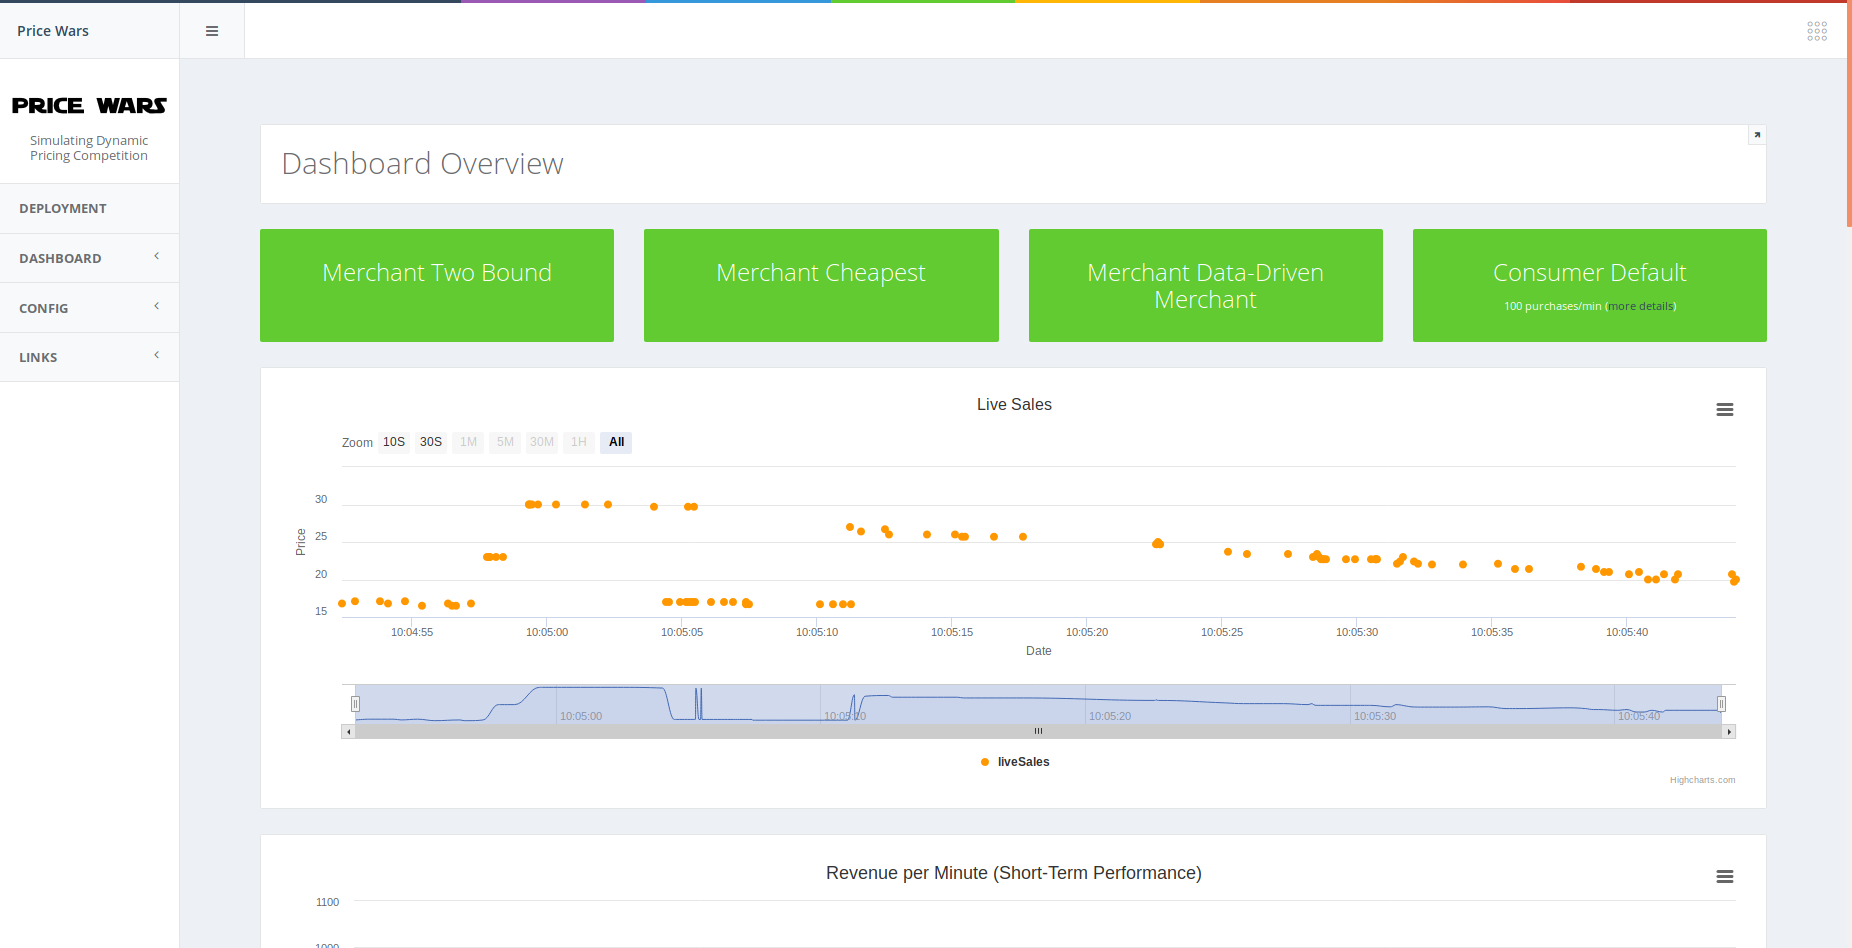
\includegraphics[width=\textwidth]{figures/dashboard}
	\caption[Screenshot of the \pricewars Dashboard]{Screenshot of the \pricewars dashboard showing participating merchants, consumers, and a sales chart. Outside the screenshot are additional charts that visualize total profit per merchant, profit per minute, revenue per hour and minute, and market share.}
	\label{fig:dashboard}
\end{figure}

%motivation! -> warum diese architecture?

The \pricewars platform is an open-source framework to simulate dynamic pricing competition on online marketplaces~\cite{DBLP:conf/recsys/0001SPSBLLSU17, edoc2017pricewars}.
Users can register their merchant on the platform to participate on the marketplace.
The platform is a sandbox environment, which can be used to test and evaluate pricing strategies under different conditions.
Developing and testing own pricing strategies can be time-consuming and possibly costly on a real online marketplace.
The platform provides an HTML-based web user interface (UI) that allows users to configure and interact with the simulation.
For example, they can explore how merchants react to a sudden increase in demand during the simulation.

The \ui includes a dashboard that visualizes price trajectories and several metrics, e.g., revenue and profit over time.
The dashboard allows to observe evolution of the market and compare status and actions of competing merchants.

Formerly, merchants on the \pricewars platform focused solely on making suitable pricing decisions.
We added features to the platform that also cause the ordering problem for the merchants.
The additions are explained in \cref{section:platform_extension}. 

\section{Motivation}
Testing new merchant strategies is time-consuming and potentially costly when done in production.
The \pricewars platform is a tool to test merchant strategies in a sandbox environment and to study how strategies interact under competition.
It is easy to set up and simulate different scenarios.
Data-driven merchants are supported by providing datasets of past sales and market situations.
The \pricewars platform is used for teaching purposes at the Hasso Plattner Institute.

\section{Services and Agents}
The \pricewars platform consists of multiple services and agents, communicate over RESTful APIs with each other.
Services provide the platform's functionality and agents interact with the platform.
Agents are merchants and consumers.
Merchants and consumers can be added and removed while the platform is running.
An overview of the architecture is presented in \cref{fig:platform_architecture}.
Each service and agent is explained in detail below:

\begin{figure}[t]
	\centering
	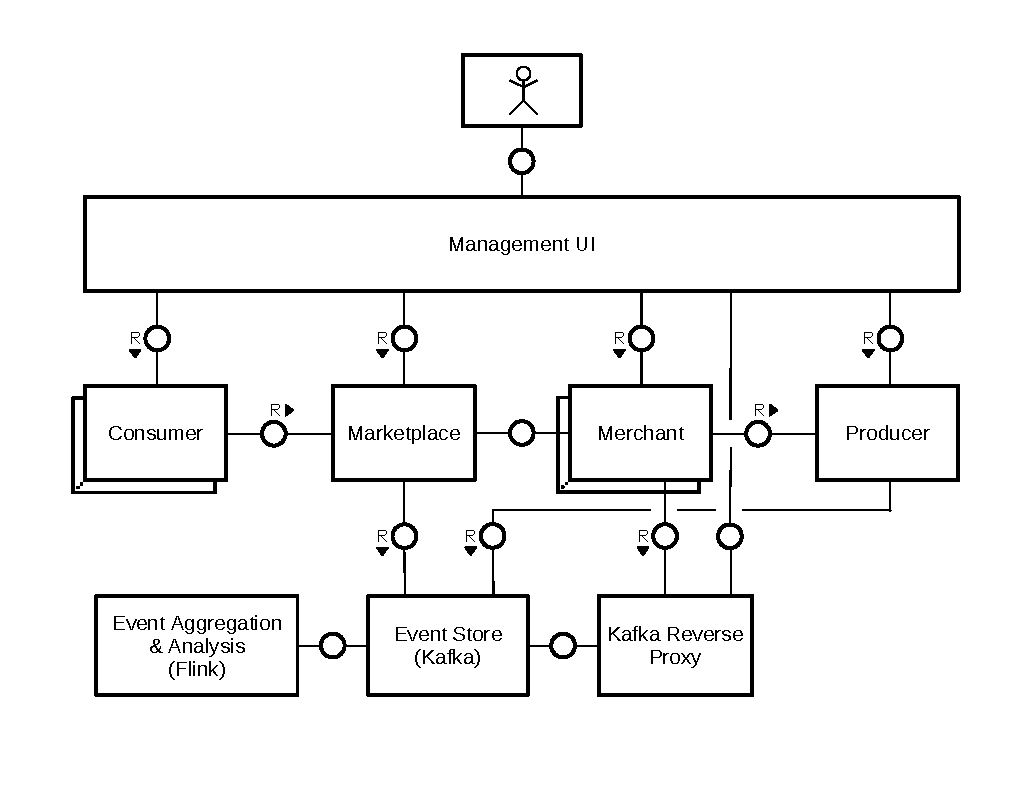
\includegraphics[width=\textwidth]{figures/pricewars-architecture}
	\caption[\pricewars Architecture]
	{Architecture of the \pricewars platform in FMC notation~\cite{knopfel2005fundamental}.}
	\label{fig:platform_architecture}
\end{figure}

%consumer/merchant can be added/removed during simulation
%use subsubsections?
\begin{description}
	\item [Marketplace]
		The marketplace is this platform's central service.
		Merchants use it to offer their products and consumers buy products on it.
		The marketplace manages merchant and consumer accounts.
		As a first step, merchants and consumers need to register on the platform, before they can perform authenticated actions like offering or buying products.
		Both, merchants and consumers can see all open offers on the marketplace.
		Merchants can adapt their prices according to competitors' prices with this information.
		Consumers inspect these offers to find their preferred offer.
		Each event that happens on the marketplace is written to a logging service.
		This data is processed to, e.g., calculate a merchant's revenue.
		Whenever a product has been sold, the marketplace notifies the selling merchant.
	\item [Merchant]
		Merchants sell products by offering them on the marketplace at a desired price.
		They can request open offers from the marketplace to adapt prices to competitors' offer prices.
		A merchant's pricing strategy can be a simple rule-based strategy like ''always undercut the cheapest competitor'' or a complex data-driven strategy that analyses the consumer behavior and/or competitors' strategies.
		Of course, also complex rule-based strategies or a hybrid of both approaches are possible.
		The \pricewars platform supports data-driven merchants by providing historical market and sales data.
		A merchant can be written in any programming language as long as the implementation complies with the platform's RESTful API.
		Documentation and an example merchant implementation is available on Github\footnote{\pricewars Merchant documentation and source code of its Python implementation on Github: \url{https://github.com/hpi-epic/pricewars-merchant}} to help users building merchants with custom strategies.
	\item [Consumer]
		The consumer agent creates a stream of consumers who visit the marketplace, inspect available offers, and buy products.
		A consumer, that does not find any acceptable offers, leaves the marketplace without buying a product.
		The consumer agent implements different buying behaviors, which can be enabled, disabled, or mixed together in the \ui.
	\item [Producer]
		A merchant can restock his inventory with new products from the producer.
		Products can be of varying quality.
		Merchants pay a certain amount of money per product.
		This amount is specified by the producer.
	\item [Web User Interface]
		The \ui allows the user to control and observe the marketplace simulation.
		Marketplace, merchants, consumer, and producer can be configured using the \ui.
		With this level of control, it is possible to test how merchants react to changing market conditions.
		For example, it can be tested how fast a merchant adapts the behavior if the consumer rate doubles.
		A dashboard contains charts that visualize merchant and consumer actions as well as merchants' short- and long-term profit and revenue.
		\cref{fig:dashboard} is a screenshot of the dashboard.
	\item [Event Processing]
	Events on the platform are processed by three separate services \textit{Apache Kafka}, \textit{Kafka Reverse Proxy}, and \textit{Apache Flink}.
	
	Apache Kafka~\cite{garg2013apache} is a stream database, which is used to store events that happen on the platform. Such events are for example orders from the producer, sales, and new offers on the marketplace.
	
	Kafka Reverse Proxy supports data-driven merchants with data about past market situations and sales.
	The data is filtered -- a merchant gets only information about his own sales -- and transformed into the CSV format.
	Additionally, the \ui gets continuous updates for its charts from the Kafka Reverse Proxy.
	
	Building onto Kafka, Apache Flink~\cite{carbone2015apache} is used to process and aggregate events to metrics like inventory level or profit per hour.
\end{description}

%write about Zookeeper: yes/no?
%Kafka requires the coordination server Apache Zookeeper.
Additionally, the marketplace uses the databases Postgres~\cite{postgres} and Redis~\cite{carlson2013redis} to manage registered accounts, product offers, and rate limiting.

\section{Deployment}
Documentation and source code of the \pricewars platform is available on Github: \url{https://github.com/hpi-epic/pricewars}.
The service-specific repositories provide instructions on how to set the services up.
Each service can be deployed on a dedicated machine this way.
Alternatively, the \pricewars platform can be deployed using docker~\cite{Merkel:2014:DLL:2600239.2600241}.
This allows an easy setup on a single machine, which is useful to try the platform out and to develop on it.
One command \texttt{docker-compose up} is enough to set up and run the whole \pricewars platform.
